\documentclass[border=10pt]{standalone}
\usepackage{pgfplots}
\pgfplotsset{compat=1.18}
\begin{document}
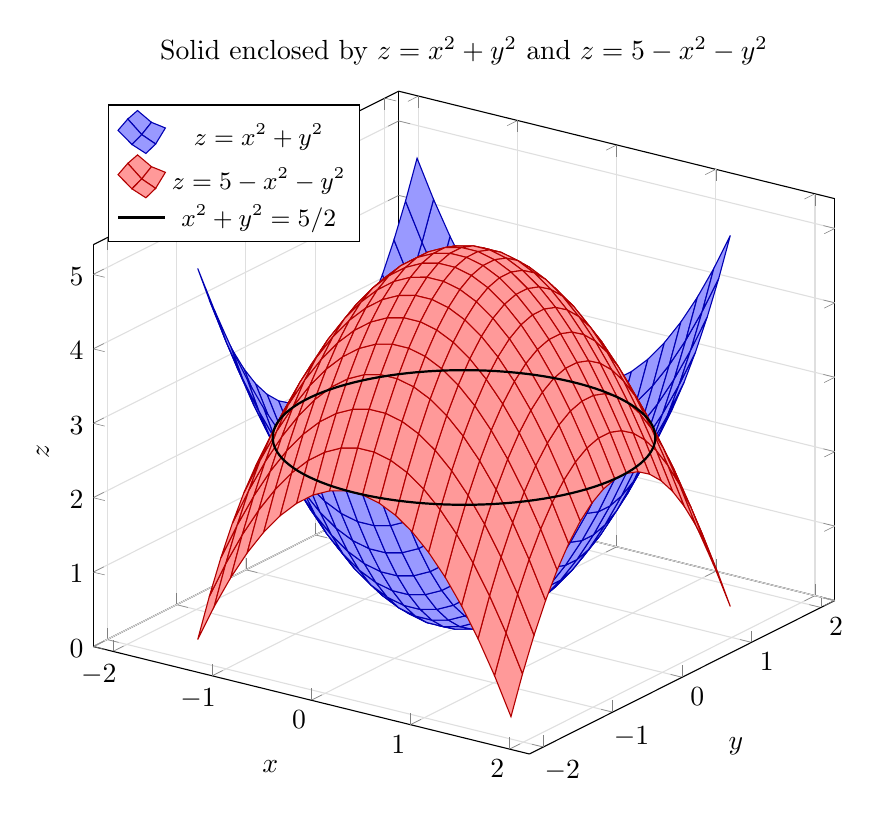
\begin{tikzpicture}
\begin{axis}[
    width=11cm, height=10cm,
    xlabel={$x$}, ylabel={$y$}, zlabel={$z$},
    view={35}{25},
    xmin=-2.2, xmax=2.2, ymin=-2.2, ymax=2.2, zmin=0, zmax=5.4,
    xtick={-2,-1,0,1,2}, ytick={-2,-1,0,1,2}, ztick={0,1,2,3,4,5},
    grid=major, grid style={gray!25},
    title={Solid enclosed by $z=x^2+y^2$ and $z=5-x^2-y^2$},
    legend style={at={(0.02,0.98)}, anchor=north west, draw=black, font=\small},
]

% Lower paraboloid: z = x^2 + y^2
\addplot3[
    surf, shader=flat,
    domain=-1.58:1.58, y domain=-1.58:1.58,
    samples=20, samples y=20,
    fill=blue!40, draw=blue!70!black,
    z buffer=sort
] {x^2 + y^2};
\addlegendentry{$z = x^2+y^2$}

% Upper paraboloid: z = 5 - x^2 - y^2
\addplot3[
    surf, shader=flat,
    domain=-1.58:1.58, y domain=-1.58:1.58,
    samples=20, samples y=20,
    fill=red!40, draw=red!70!black,
    z buffer=sort
] {5 - x^2 - y^2};
\addlegendentry{$z = 5-x^2-y^2$}

% Intersection circle: x^2+y^2 = 5/2, z = 5/2
\addplot3[
    domain=0:360, samples=120,
    samples y=1, thick, black
] ({sqrt(2.5)*cos(x)}, {sqrt(2.5)*sin(x)}, {2.5});
\addlegendentry{$x^2+y^2=5/2$}

\end{axis}
\end{tikzpicture}
\end{document}